\documentclass[tikz,border=10pt]{standalone}
\usetikzlibrary{arrows.meta, positioning, shapes.geometric}

\begin{document}
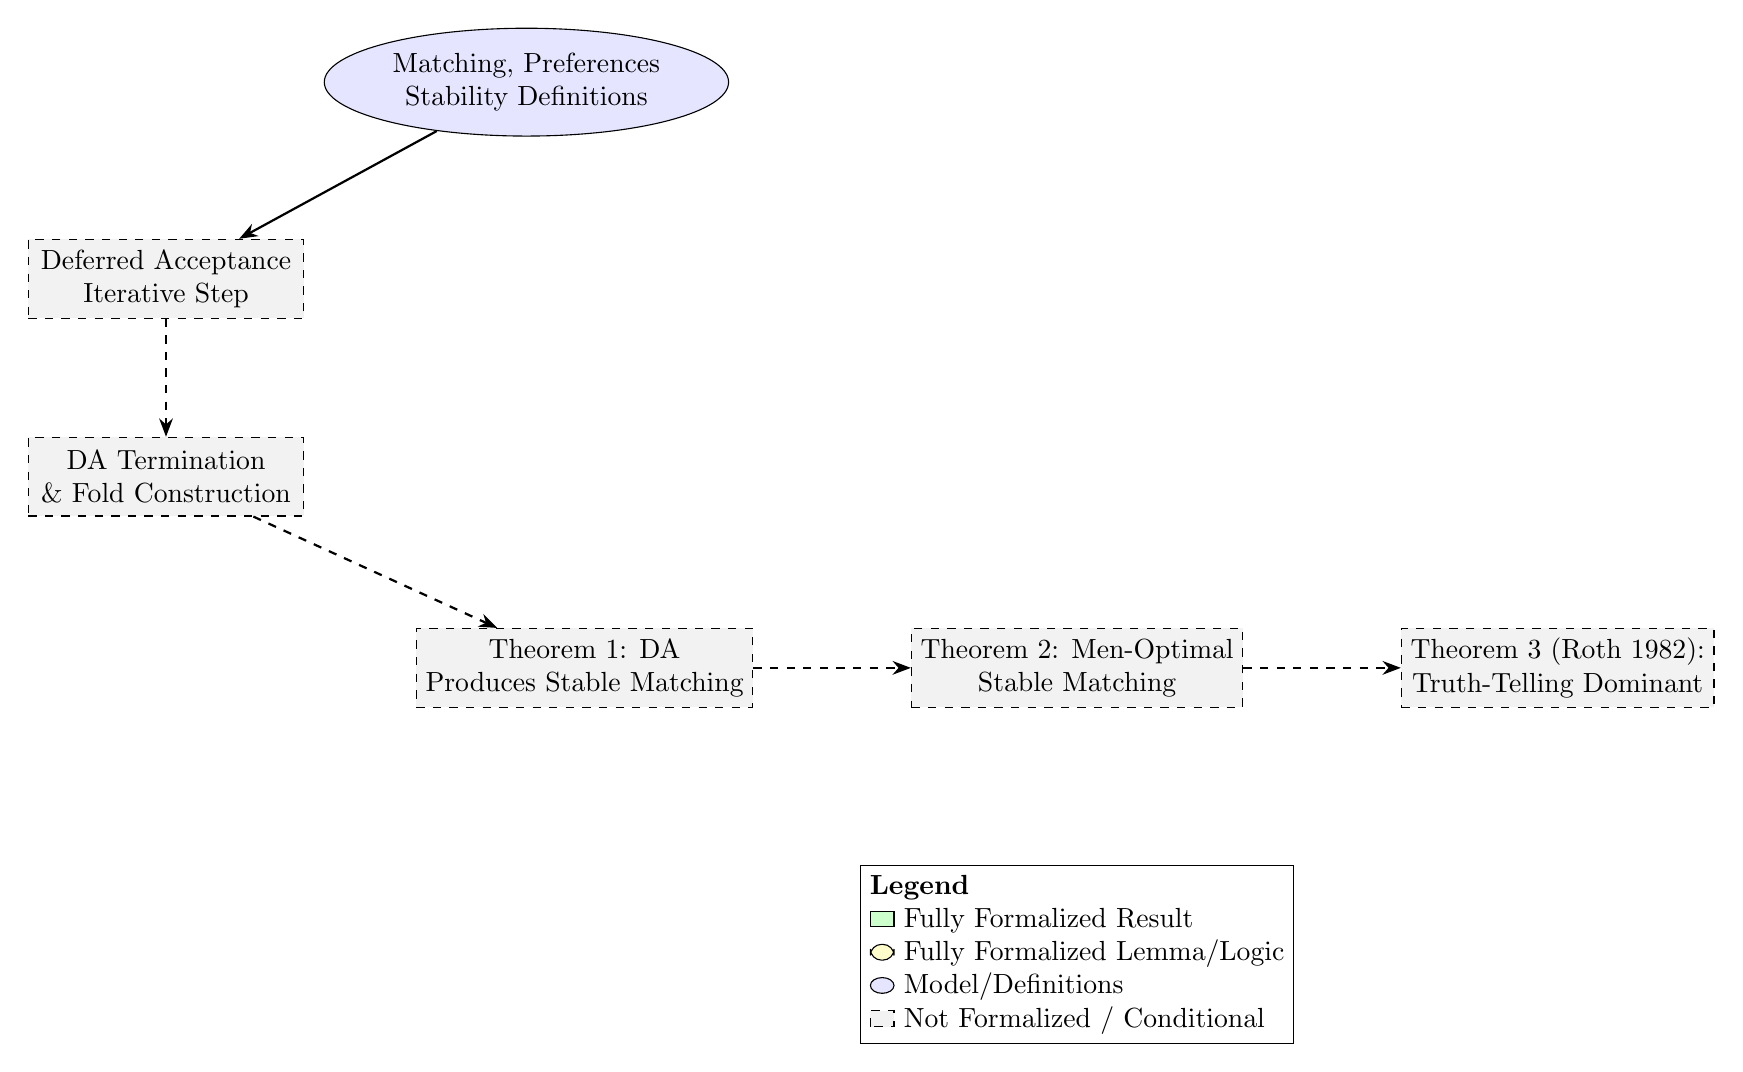
\begin{tikzpicture}[
    node distance=1.5cm and 2cm,
    result/.style={rectangle, draw, fill=green!20, minimum width=3.5cm, minimum height=1cm, align=center},
    model/.style={ellipse, draw, fill=blue!10, minimum width=3cm, minimum height=1cm, align=center},
    lemma/.style={rectangle, draw, fill=yellow!20, minimum width=3.5cm, minimum height=1cm, align=center, rounded corners},
    unformalized/.style={rectangle, draw, dashed, fill=gray!10, minimum width=3.5cm, minimum height=1cm, align=center},
    arrow/.style={-{Stealth}, thick}
]

% Center Column (Definitions)
\node[model] (Primitives) {Matching, Preferences \\ Stability Definitions};

% Left Column (Algorithm)
\node[unformalized, below left=1.5cm and 1cm of Primitives] (DA_Step) {Deferred Acceptance \\ Iterative Step};
\node[unformalized, below=of DA_Step] (DA_Term) {DA Termination \\ \& Fold Construction};

% Results
\node[unformalized, below right=2cm of DA_Term] (Thm1) {Theorem 1: DA \\ Produces Stable Matching};
\node[unformalized, right=of Thm1] (Thm2) {Theorem 2: Men-Optimal \\ Stable Matching};
\node[unformalized, right=of Thm2] (Thm3) {Theorem 3 (Roth 1982): \\ Truth-Telling Dominant};

% Edges
\draw[arrow] (Primitives) -- (DA_Step);
\draw[arrow, dashed] (DA_Step) -- (DA_Term);
\draw[arrow, dashed] (DA_Term) -- (Thm1);
\draw[arrow, dashed] (Thm1) -- (Thm2);
\draw[arrow, dashed] (Thm2) -- (Thm3);

% Legend
\node[draw, rectangle, below=2cm of Thm2, align=left] (Legend) {
    \textbf{Legend} \\
    \tikz\draw[fill=green!20] (0,0) rectangle (0.3,0.2); Fully Formalized Result \\
    \tikz\draw[fill=yellow!20, rounded corners] (0,0) rectangle (0.3,0.2); Fully Formalized Lemma/Logic \\
    \tikz\draw[fill=blue!10] (0,0) ellipse (0.15 and 0.1); Model/Definitions \\
    \tikz\draw[dashed, fill=gray!10] (0,0) rectangle (0.3,0.2); Not Formalized / Conditional
};

\end{tikzpicture}
\end{document}